\section{Tank Monitoring Subsystem (TMS)}%
\label{sec:tms}

Il Tank Monitoring Subsystem (TMS) acquisisce periodicamente
il livello di riempimento della tanica e comunica le misure
al CUS tramite MQTT.


\subsection{Architettura software}%
\label{subsec:tms-architecture}

Il firmware è organizzato in due task FreeRTOS eseguiti
su core distinti.
La separazione tra acquisizione e comunicazione permette
di proseguire le misurazioni anche durante l'attesa
o il recupero della connessione.
La Tabella~\ref{tab:tms-tasks} riassume le responsabilità
dei due task.

\begin{table}[H]
    \centering

    \begin{tabularx}{\linewidth}{
        @{}l >{\raggedright\arraybackslash}X@{}
    }
        \toprule
        \textbf{Task} &
        \textbf{Responsabilità principale} \\
        \midrule

        \texttt{WaterLevelTask} &
        Acquisizione e validazione delle letture,
        calcolo del livello di riempimento. \\

        \texttt{CommunicationTask} &
        Gestione Wi-Fi e MQTT, pubblicazione dei dati
        e aggiornamento dei LED di stato. \\

        \bottomrule
    \end{tabularx}

    \caption{Task principali del firmware TMS.}
    \label{tab:tms-tasks}
\end{table}

Lo scambio dei dati avviene tramite una coda condivisa
che contiene una sola misura.
Ogni nuova lettura sostituisce quella eventualmente
non ancora trasmessa, così che al ripristino della
comunicazione sia disponibile il dato più recente,
senza accumulare uno storico da inviare.

I collegamenti hardware e i parametri operativi
sono centralizzati nel file \texttt{config.h}.
Eventuali errori nella creazione delle risorse RTOS
vengono rilevati e segnalati durante l'avvio.


\subsection{Circuito e componenti hardware}%
\label{subsec:tms-hardware}

Il prototipo comprende una scheda ESP32, un sonar
HC-SR04 e due LED, verde e rosso, per la segnalazione
dello stato della comunicazione.
I collegamenti sono realizzati su breadboard,
come mostrato nella Figura~\ref{fig:tms-wiring}.

\begin{figure}[H]
    \centering

    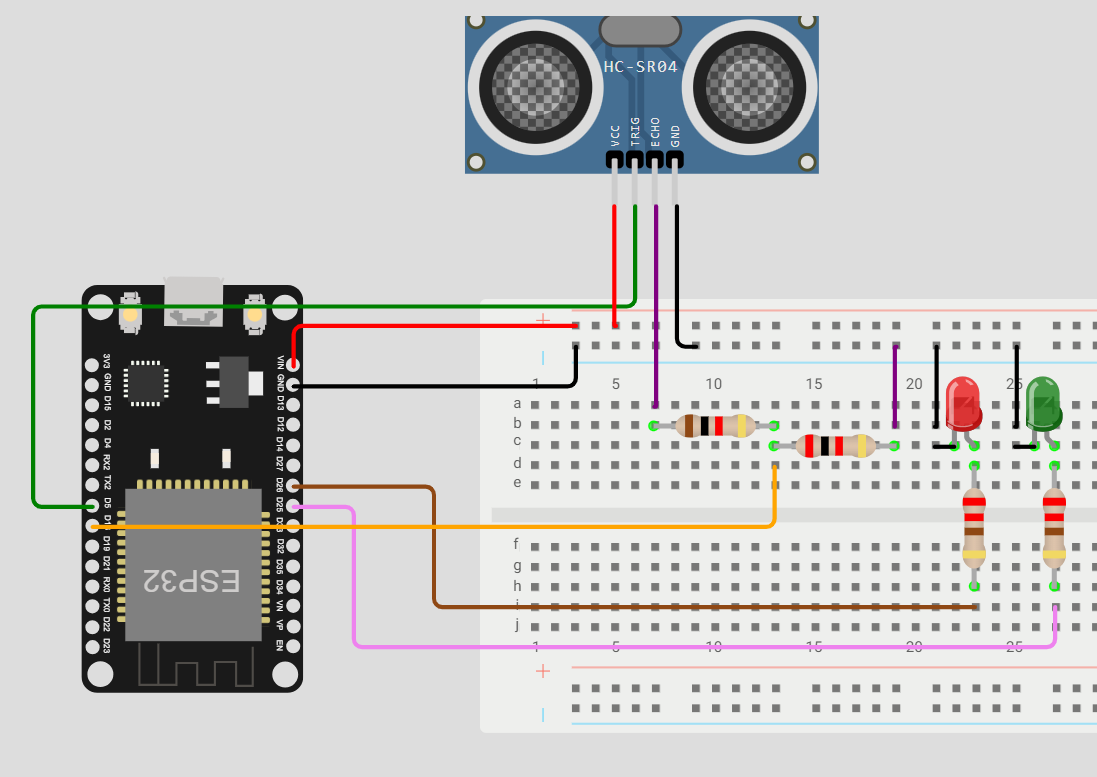
\includegraphics[
        width=0.64\linewidth
    ]{figures/tms_wiring.png}

    \caption{Cablaggio del TMS: ESP32, sonar HC-SR04 e LED di stato.}
    \label{fig:tms-wiring}
\end{figure}

La Tabella~\ref{tab:tms-pins} riassume l'assegnazione dei segnali.

\begin{table}[H]
    \centering

    \begin{tabularx}{\linewidth}{
        @{}l >{\raggedright\arraybackslash}X@{}
    }
        \toprule
        \textbf{GPIO} & \textbf{Collegamento} \\
        \midrule

        5  & Segnale TRIG del sonar \\

        18 & Segnale ECHO del sonar, attraverso il partitore resistivo \\

        25 & LED verde \\

        26 & LED rosso \\

        \bottomrule
    \end{tabularx}

    \caption{Assegnazione dei GPIO del TMS.}
    \label{tab:tms-pins}
\end{table}

Il segnale ECHO è adattato agli ingressi a
\(3{,}3\,\mathrm{V}\) dell'ESP32 mediante un partitore
resistivo da \(1\,\mathrm{k}\Omega\) e
\(2\,\mathrm{k}\Omega\).
Ogni LED utilizza una resistenza in serie
da \(220\,\Omega\) per limitare la corrente.


\subsection{Task del firmware}%
\label{subsec:tms-tasks}


\subsubsection{CommunicationTask}%
\label{subsec:tms-communication}

La logica di comunicazione è descritta da una macchina
a stati finiti che distingue le fasi di connessione
dalla condizione operativa.

Gli stati principali sono:

\begin{itemize}
    \item \texttt{WIFI\_CONNECTING}: attesa della
    connessione alla rete Wi-Fi

    \item \texttt{MQTT\_CONNECTING}: connessione
    al broker MQTT

    \item \texttt{WAITING\_FIRST\_PUBLISH}: connessione
    MQTT stabilita, in attesa della prima pubblicazione
    riuscita

    \item \texttt{COMMUNICATION\_OK}: comunicazione
    operativa dopo la prima pubblicazione riuscita
\end{itemize}

La Figura~\ref{fig:tms-communication-fsm} mostra
la macchina a stati del task.

\begin{landscape}
    \begin{figure}[p]
        \centering

        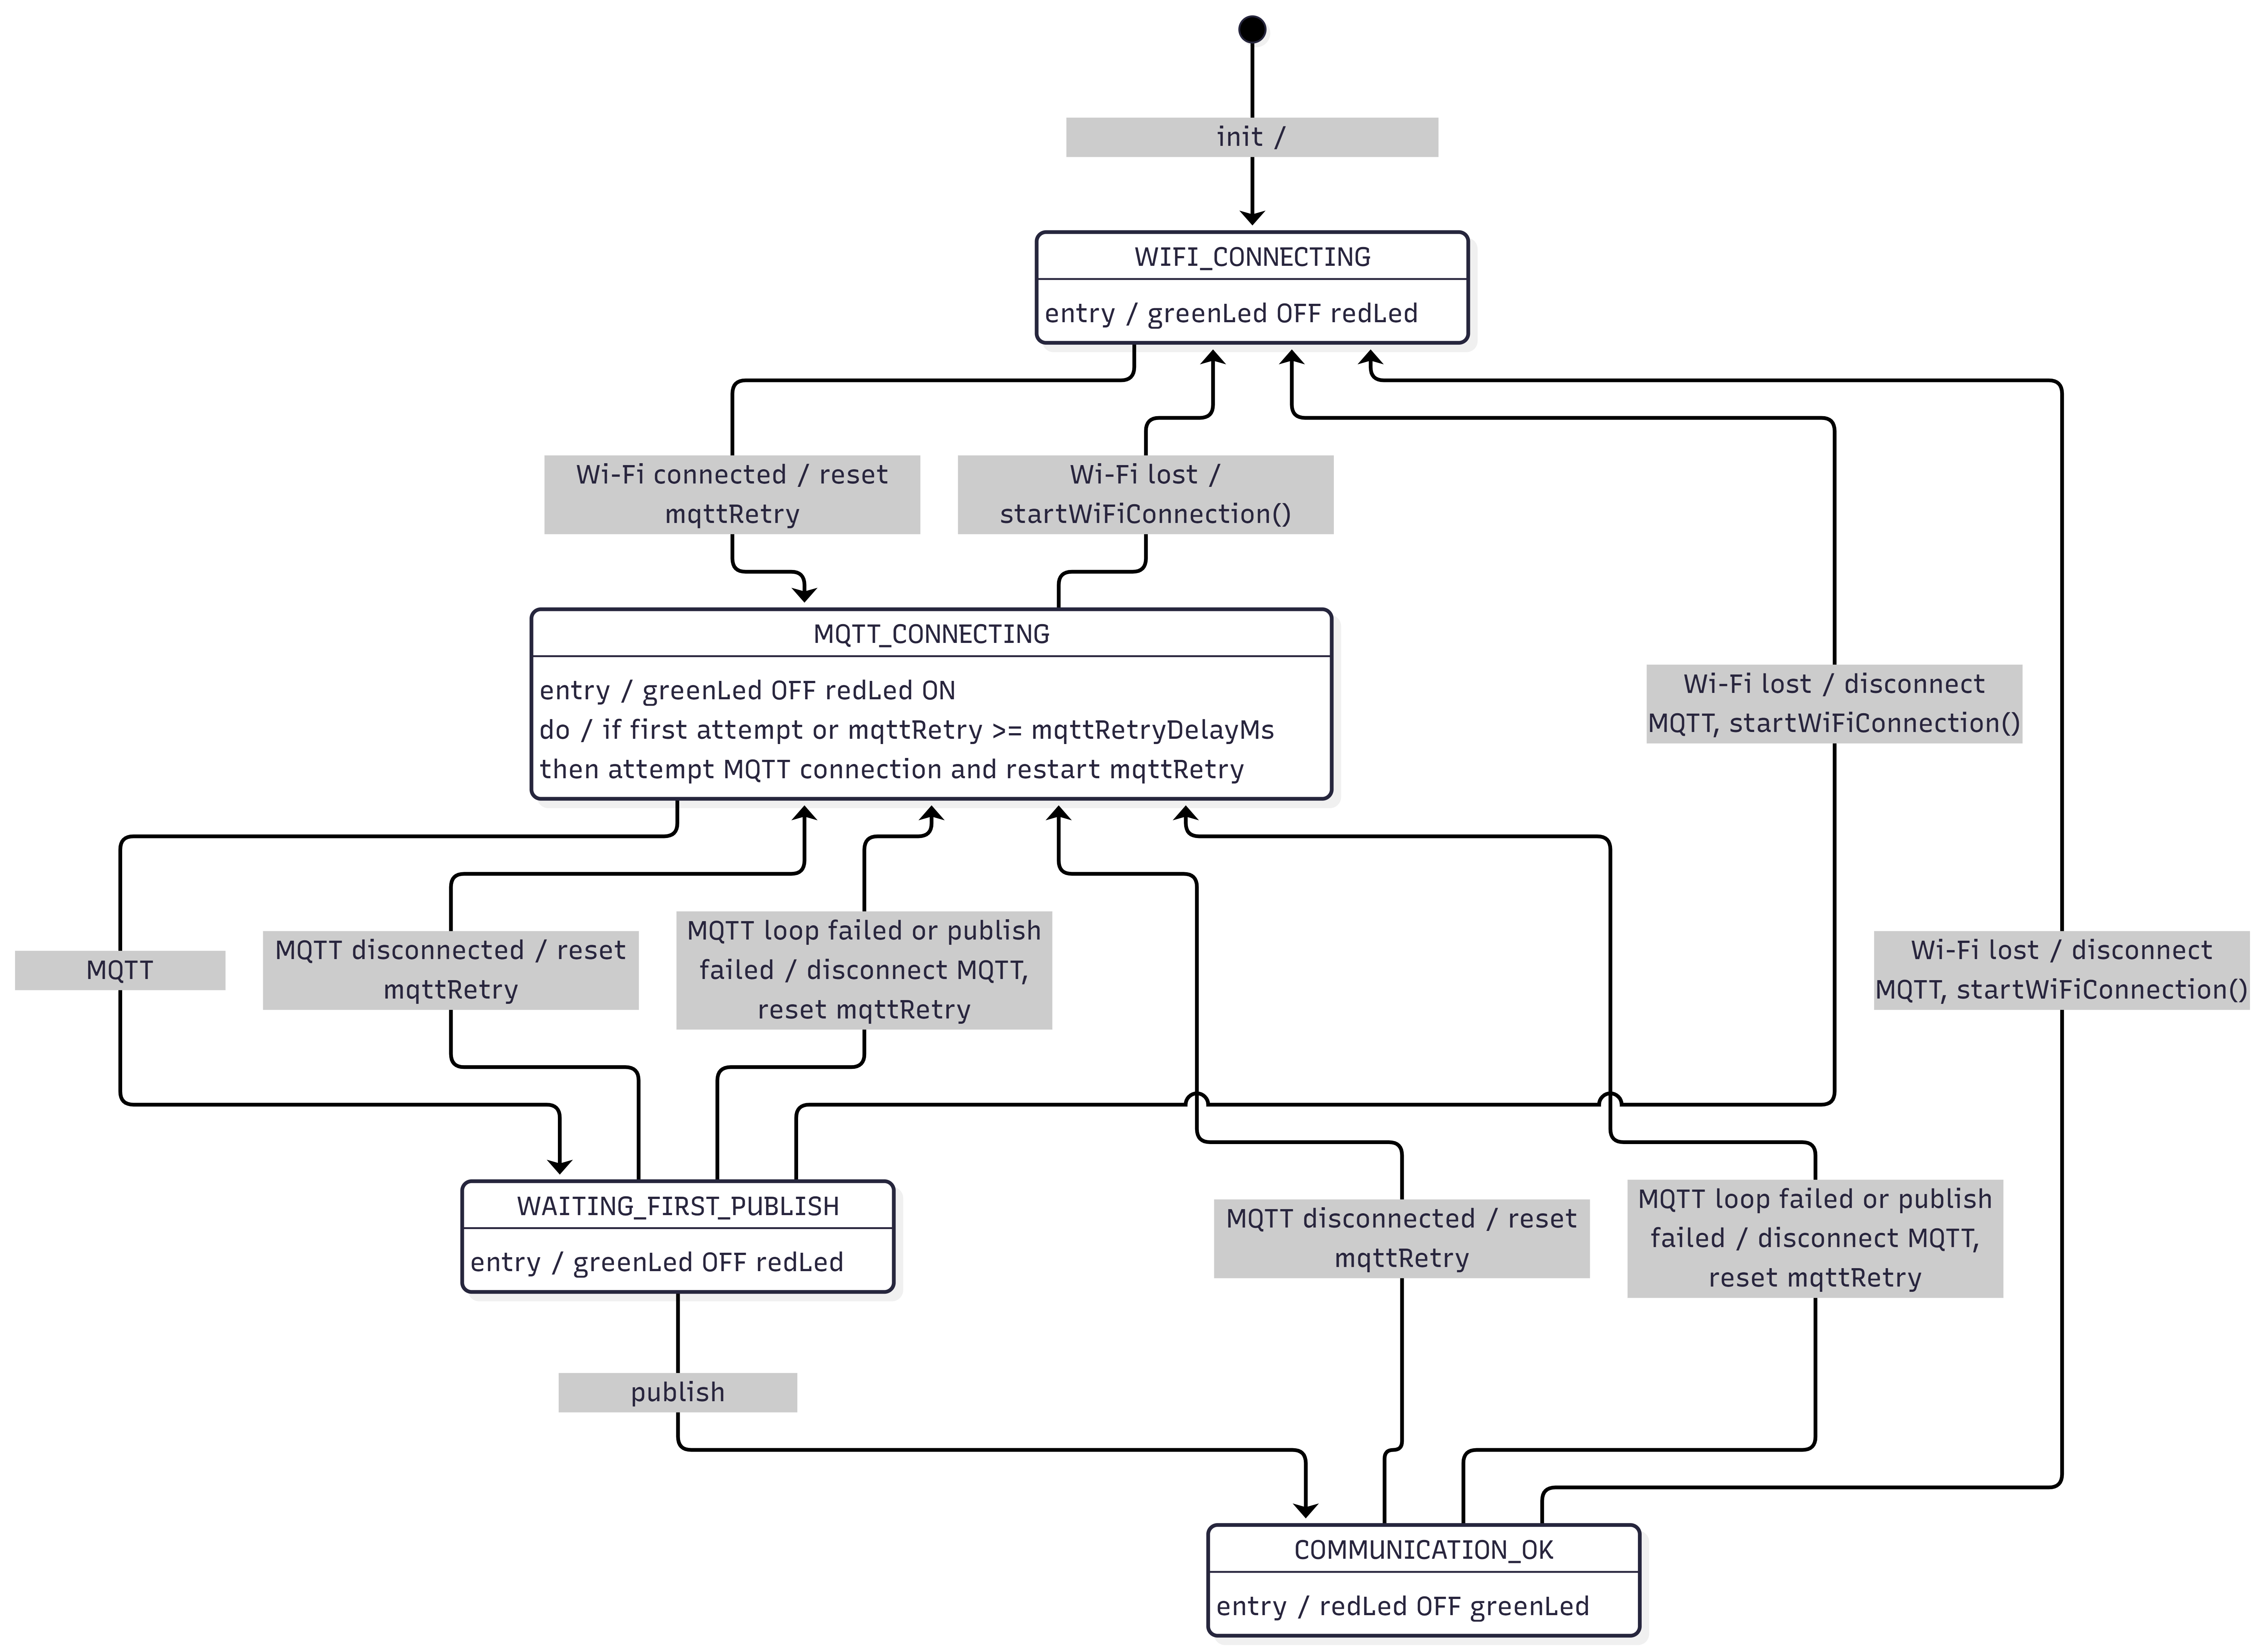
\includegraphics[
            width=\linewidth,
            height=0.90\textheight,
            keepaspectratio
        ]{figures/communication_fsm.png}

        \caption{FSM del CommunicationTask.}%
        \label{fig:tms-communication-fsm}
    \end{figure}
\end{landscape}

Il task pubblica l'ultima lettura disponibile e mantiene
attiva la comunicazione.
La perdita del Wi-Fi riporta alla fase di connessione
alla rete.
Se il Wi-Fi è disponibile, un'interruzione MQTT
o un errore di pubblicazione attiva la riconnessione
al broker.
I tentativi successivi sono separati da un intervallo
configurabile.

Il LED verde è acceso e quello rosso è spento
nella condizione operativa; negli altri stati
la segnalazione è invertita.
Dopo una disconnessione, il verde viene riacceso
soltanto a seguito di una nuova pubblicazione riuscita.
I LED rappresentano lo stato della comunicazione,
indipendentemente dalla validità della lettura trasmessa.

Il CUS riceve i messaggi JSON sottoscrivendo
lo stesso topic utilizzato dal TMS.
Per una misura valida vengono trasmessi il livello
in metri e la percentuale di riempimento:

\begin{verbatim}
{"status":"OK","levelM":0.150,"percentage":50.0}
\end{verbatim}

Una lettura non valida viene segnalata mediante:

\begin{verbatim}
{"status":"NO_ECHO"}
\end{verbatim}


\subsubsection{WaterLevelTask}%
\label{subsec:tms-water-level}

Il task acquisisce periodicamente la distanza dalla
superficie dell'acqua e calcola il livello
di riempimento.
Il periodo di campionamento è configurabile.

Nel modello adottato, il piano del sensore rappresenta
il riempimento al \(100\%\).
Indicando con \(H\) la distanza tra il sensore
e il fondo della tanica e con \(d\) la distanza
dalla superficie dell'acqua, il livello \(h\)
e la percentuale \(p\) sono calcolati come:

\[
    h = H - d,
    \qquad
    p = \frac{h}{H} \cdot 100
\]

La lettura è considerata valida se l'eco viene rilevato
e la distanza soddisfa \(0 \leq d \leq H\).
Il livello risultante è quindi compreso tra zero
e \(H\), mentre la percentuale appartiene
all'intervallo tra \(0\%\) e \(100\%\).

Le letture senza eco o fuori intervallo vengono
classificate come non valide e il livello
non viene calcolato.
Anche questo esito viene reso disponibile al task
di comunicazione, distinguendolo dalla condizione
di tanica vuota, che corrisponde invece a una lettura
valida con \(d = H\).


\subsection{Test, criticità e taratura}%
\label{subsec:tms-tests}

\paragraph{Allestimento e verifica delle misure.}

Le prove sono state effettuate spostando una scatolina
in polimero di forma geometrica regolare davanti
al sonar, simulando diversi livelli di riempimento.
L'altezza utile è stata configurata a
\(0{,}30\,\mathrm{m}\), corrispondenti alla lunghezza
del righello utilizzato come riferimento;
il periodo di acquisizione è stato impostato
a \(2\,\mathrm{s}\).

Le distanze rilevate sono risultate approssimativamente
corrispondenti a quelle misurate con il righello,
fornendo una verifica qualitativa dell'acquisizione.
È stata inoltre verificata la coerenza tra livello
espresso in metri e percentuale di riempimento.

\paragraph{Gestione delle letture non valide.}

Durante le prove preliminari con la mano come bersaglio
sono state osservate letture \texttt{NO\_ECHO};
è stato quindi utilizzato un oggetto di forma regolare
per proseguire le verifiche.

La classificazione delle letture fuori intervallo
è stata controllata posizionando il bersaglio
oltre i \(30\,\mathrm{cm}\).
Le letture sono state segnalate come non valide.
Il CUS ha riconosciuto i messaggi \texttt{NO\_ECHO}
e restituito \texttt{null} per la misura non disponibile,
distinguendola da un livello valido pari a zero.

\paragraph{Avvio e recupero della comunicazione.}

All'avvio e dopo un riavvio mediante il pulsante RESET
è stata osservata l'accensione iniziale del LED rosso,
seguita dal passaggio al verde al ripristino
della comunicazione.

È stato inoltre verificato il recupero dopo
un'interruzione del Wi-Fi mantenendo la scheda accesa.
Al ripristino della rete, il TMS ha ristabilito
automaticamente la comunicazione ed è tornato
alla segnalazione verde, senza richiedere
un riavvio manuale.
